\subsection{主结果}

表~\ref{tab:main} 与图~\ref{fig:main} 汇总 11 个条件。闭卷 C0 的归一化正确率为 0.225（严格正确 7\%），说明该 gold set 基本无法依靠 7B 模型的参数记忆回答。加入检索后，NaiveRAG（C1）达到 0.820，完整 LightRAG（C2）为 0.845；C2 相对 C1 的配对差为 $+0.025$（95\% CI $[-0.040,0.090]$，$p=0.515$），在 100 题上不构成显著差异。C8（抽取式画像）与 C9（时序图）分别为 0.865 与 0.870，C4（仅高层）为 0.845，C3（仅低层）为 0.820。最低的检索条件是 C5（去原文），正确率为 0.445，相对 C2 低 0.400（95\% CI $[0.310,0.490]$，$p<0.001$），拒答率升至 47\%。

\begin{figure}[H]
\centering
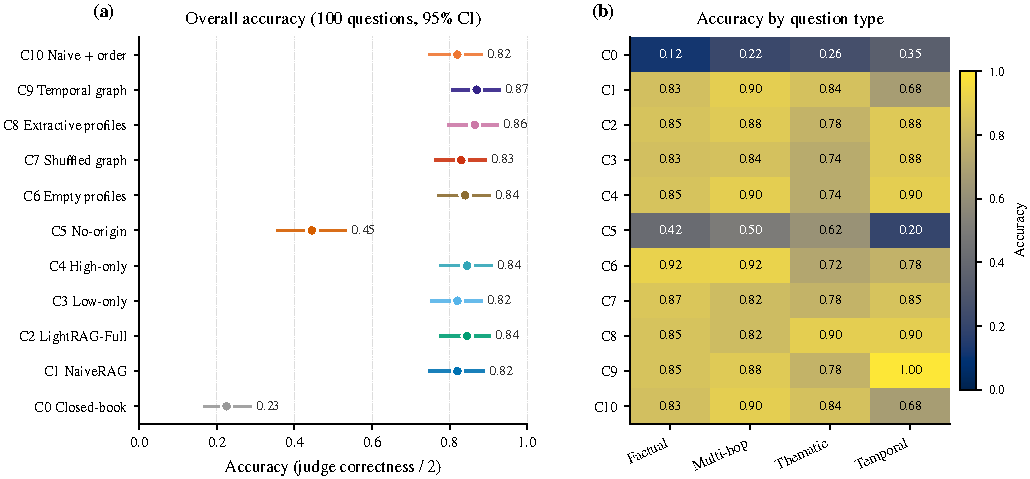
\includegraphics[width=\textwidth]{figures/fig1_main.pdf}
\caption{总体正确率与分题型正确率。(a) judge correctness/2 的均值与 95\% bootstrap CI。(b) 分题型正确率热图；颜色越亮表示越高。}
\label{fig:main}
\end{figure}

\begin{table}[H]
\centering
\caption{总体结果（100 题，均值与 95\% bootstrap CI）。}
\label{tab:main}
\scriptsize
\setlength{\tabcolsep}{3.0pt}
\begin{threeparttable}
\begin{tabular}{@{}l r c c c c c c c c r@{}}
\toprule
Condition & $n$ & Accuracy [95\% CI] & Strict & Lenient & F1 & Cite-P & Cite-R & Refusal & Evid-R & Ctx \\
\midrule
C0 & 100 & 0.23 [0.17, 0.29] & 0.07 & 0.38 & 0.06 & -- & 0.00 & 0.00 & 0.00 & -- \\
C1 & 100 & 0.82 [0.74, 0.89] & 0.79 & 0.85 & 0.20 & 0.98 & 0.54 & 0.12 & 0.86 & 2862 \\
C2 & 100 & 0.84 [0.78, 0.91] & 0.81 & 0.88 & 0.19 & 0.96 & 0.61 & 0.10 & 0.78 & 2853 \\
C3 & 100 & 0.82 [0.75, 0.89] & 0.78 & 0.86 & 0.19 & 0.95 & 0.60 & 0.10 & 0.79 & 2830 \\
C4 & 100 & 0.84 [0.78, 0.91] & 0.82 & 0.87 & 0.18 & 0.98 & 0.58 & 0.12 & 0.78 & 2849 \\
C5 & 100 & 0.45 [0.35, 0.54] & 0.39 & 0.50 & 0.09 & 0.89 & 0.34 & 0.47 & 0.00 & 2900 \\
C6 & 100 & 0.84 [0.77, 0.91] & 0.80 & 0.88 & 0.19 & 0.99 & 0.61 & 0.11 & 0.78 & 2846 \\
C7 & 100 & 0.83 [0.76, 0.90] & 0.79 & 0.87 & 0.18 & 0.95 & 0.60 & 0.09 & 0.78 & 2849 \\
C8 & 100 & 0.86 [0.80, 0.93] & 0.84 & 0.89 & 0.20 & 0.97 & 0.57 & 0.05 & 0.78 & 2845 \\
C9 & 100 & 0.87 [0.81, 0.93] & 0.84 & 0.90 & 0.21 & 0.97 & 0.64 & 0.08 & 0.80 & 2854 \\
C10 & 100 & 0.82 [0.74, 0.89] & 0.79 & 0.85 & 0.21 & 0.98 & 0.56 & 0.12 & 0.86 & 2862 \\
\bottomrule
\end{tabular}
\begin{tablenotes}\scriptsize
\item 正确率为 judge correctness / 2，Strict 为 2，Lenient 为 $\ge$ 1，Cite-P/R 为引用精确率/召回率，Refusal 为回答“上下文不足”的比例，Evid-R 为 gold 证据诗节进入上下文的比例，Ctx 为估计上下文 token。C0--C10 见表~\ref{tab:conditions}。
\end{tablenotes}
\end{threeparttable}
\end{table}


\begin{table}[H]
\centering
\caption{分题型正确率（judge correctness / 2）。}
\label{tab:types}
\small
\begin{threeparttable}
\begin{tabular}{@{}l cccc@{}}
\toprule
Condition & Factual (30) & Multi-hop (25) & Thematic (25) & Temporal (20) \\
\midrule
C0 & 0.12 & 0.22 & 0.26 & 0.35 \\
C1 & 0.83 & 0.90 & 0.84 & 0.68 \\
C2 & 0.85 & 0.88 & 0.78 & 0.88 \\
C3 & 0.83 & 0.84 & 0.74 & 0.88 \\
C4 & 0.85 & 0.90 & 0.74 & 0.90 \\
C5 & 0.42 & 0.50 & 0.62 & 0.20 \\
C6 & 0.92 & 0.92 & 0.72 & 0.78 \\
C7 & 0.87 & 0.82 & 0.78 & 0.85 \\
C8 & 0.85 & 0.82 & 0.90 & 0.90 \\
C9 & 0.85 & 0.88 & 0.78 & 1.00 \\
C10 & 0.83 & 0.90 & 0.84 & 0.68 \\
\bottomrule
\end{tabular}
\begin{tablenotes}\scriptsize
\item 数值为均值，95\% CI 见图~\ref{fig:main}(b) 与补充表。
\end{tablenotes}
\end{threeparttable}
\end{table}


\subsection{H1 图结构还是 LLM 画像文本}

图~\ref{fig:attribution}(a) 与表~\ref{tab:paired} 给出 H1 的配对比较。四个关键对照均无显著差异。

\begin{itemize}
\item C2 相对 C6（置空 LLM 画像）为 $+0.005$，95\% CI $[-0.040,0.050]$，$p=0.908$；
\item C2 相对 C7（打乱一跳结构）为 $+0.015$，95\% CI $[-0.035,0.065]$，$p=0.638$；
\item C6 相对 C1（图结构但无 LLM 画像）为 $+0.020$，95\% CI $[-0.050,0.090]$，$p=0.614$；
\item C2 相对 C1 为 $+0.025$，95\% CI $[-0.040,0.090]$，$p=0.515$。
\end{itemize}

C2 相对 C5（去除原始 chunk）高 0.400，95\% CI $[0.310,0.490]$，$p<0.001$；C0 相对 C1 低 0.595，95\% CI $[-0.685,-0.500]$，$p<0.001$。C3 与 C4 的差异也不显著（C2$-$C3 $+0.025$，$p=0.148$；C2$-$C4 $0.000$，$p=1.000$）。

\begin{figure}[H]
\centering
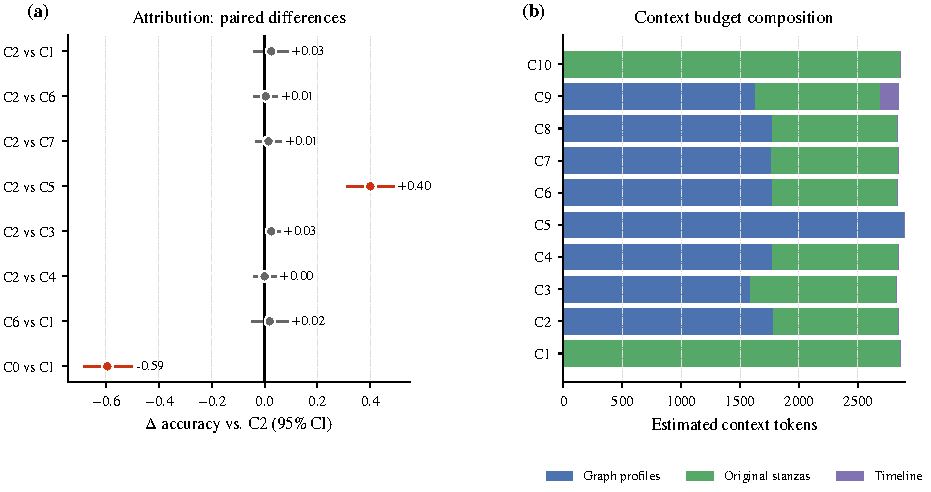
\includegraphics[width=\textwidth]{figures/fig2_attribution.pdf}
\caption{归因与上下文构成。(a) 相对完整 LightRAG（C2）的配对正确率差与 95\% CI；红色表示 Holm 校正后 $p<0.05$。(b) 估计的上下文 token 构成。}
\label{fig:attribution}
\end{figure}

\begin{table}[H]
\centering
\caption{相对完整 LightRAG（C2）的配对差异、95\% CI 与 Holm 校正 $p$ 值。}
\label{tab:paired}
\scriptsize
\setlength{\tabcolsep}{3.0pt}
\begin{threeparttable}
\begin{tabular}{@{}l l l c c c c r@{}}
\toprule
Family & Comparison & Scope & $\Delta$ accuracy & 95\% CI & $p$ & $p_{\mathrm{Holm}}$ & $n$ \\
\midrule
H1 & C2 $-$ C1 & All & 0.025 & [-0.040, 0.090] & 0.5154 & 1.0000 & 100 \\
H1 & C2 $-$ C6 & All & 0.005 & [-0.040, 0.050] & 0.9084 & 1.0000 & 100 \\
H1 & C2 $-$ C7 & All & 0.015 & [-0.035, 0.065] & 0.6376 & 1.0000 & 100 \\
H1 & C2 $-$ C5 & All & 0.400 & [0.310, 0.490] & 0.0000 & 0.0000 & 100 \\
H1 & C2 $-$ C3 & All & 0.025 & [-0.005, 0.060] & 0.1484 & 0.8904 & 100 \\
H1 & C2 $-$ C4 & All & 0.000 & [-0.040, 0.045] & 1.0000 & 1.0000 & 100 \\
H1 & C6 $-$ C1 & All & 0.020 & [-0.050, 0.090] & 0.6138 & 1.0000 & 100 \\
H1 & C0 $-$ C1 & All & -0.595 & [-0.685, -0.500] & 0.0000 & 0.0000 & 100 \\
H2 & C2 $-$ C8 & Accuracy & -0.020 & [-0.085, 0.045] & 0.5874 & 1.0000 & 100 \\
H2 & C2 $-$ C8 & Cite-P & -0.002 & [-0.034, 0.026] & 0.9082 & 1.0000 & 81 \\
H2 & C2 $-$ C8 & Unsupported & -0.015 & [-0.072, 0.039] & 0.5936 & 1.0000 & 92 \\
H3 & C9 $-$ C2 & Temporal & 0.125 & [0.000, 0.275] & 0.0768 & 0.1536 & 20 \\
H3 & C9 $-$ C10 & Temporal & 0.325 & [0.150, 0.525] & 0.0000 & 0.0000 & 20 \\
H3 & C10 $-$ C1 & Temporal & 0.000 & [-0.150, 0.150] & 1.0000 & 1.0000 & 20 \\
H3 & C2 $-$ C1 & Temporal & 0.200 & [0.050, 0.375] & 0.0050 & 0.0150 & 20 \\
\bottomrule
\end{tabular}
\begin{tablenotes}\scriptsize
\item 正的 $\Delta$ 表示前一个条件更准确。H1 检验图与画像的归因，H2 检验改写偏差，H3 检验时序表示。C9/C10 的比较只用 20 道时序题。
\end{tablenotes}
\end{threeparttable}
\end{table}


该结果直接回应了该博客的第一项批评。在该语料上，去掉 LLM 画像文本（C6）或打乱图结构（C7）均未使正确率显著下降，图结构也未让 C2 显著高于 NaiveRAG。条件差异主要与原始 chunk 是否进入上下文相关。C5 去掉原文后，正确率由 0.845 降至 0.445，拒答率由 10\% 升至 47\%，citation recall 由 0.61 降至 0.34。图画像文本未能替代原始 chunk，反而在上下文预算中占用部分原文空间。C2 的 gold 证据召回为 0.78，低于 C1 的 0.86；C2 的上下文由约 1,784 token 图画像与 1,064 token 原文组成，C1 的 2,862 token 几乎全是原文。图结构带来的 citation recall 提升确实存在（C2 0.61 对 C1 0.54），但未转化为正确率。

\subsection{H2 改写偏差与可回溯性}

H2 的结果为部分成立，方向与该博客的强版本判断不同。对画像事实性的审计（表~\ref{tab:profiles}、图~\ref{fig:factuality}(a)）显示，LLM 画像的实体支持率为 0.952（SD 0.130），高于抽取式画像的 0.883（SD 0.150）；关系支持率分别为 0.871（SD 0.195）与 0.877（SD 0.181）。答案层亦未出现 LLM 画像导致引用精确率下降的现象。C2 的 citation precision 为 0.963，C8 为 0.969；unsupported claim rate 分别为 0.094 与 0.109；C2$-$C8 在正确率、citation precision、unsupported claim rate 上的配对差分别为 $-0.020$（$p=0.587$）、$-0.002$（$p=0.912$）、$-0.015$（$p=0.594$）。

\begin{figure}[H]
\centering
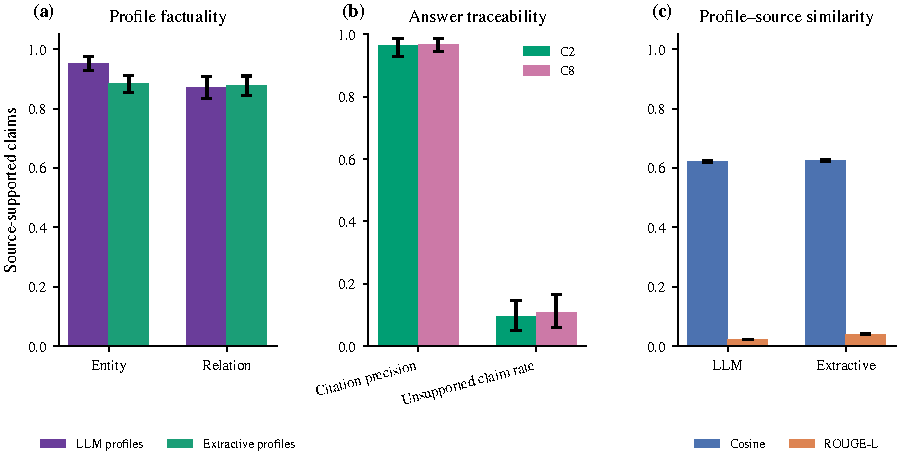
\includegraphics[width=\textwidth]{figures/fig3_factuality.pdf}
\caption{画像事实性、答案可回溯性与画像--原文相似度。(a) 被源诗节支持的画像断言比例。(b) 引用精确率与 unsupported claim rate。(c) 画像与源诗节的 cosine 与 ROUGE-L。}
\label{fig:factuality}
\end{figure}

\begin{table}[H]
\centering
\caption{画像事实性审计，被源诗节支持的原子断言比例（每格 30 条）。}
\label{tab:profiles}
\small
\begin{threeparttable}
\begin{tabular}{@{}l l r c c@{}}
\toprule
Profile & Graph element & $n$ & Support rate & SD \\
\midrule
LLM & Entity & 30 & 0.95 & 0.13 \\
LLM & Relation & 29 & 0.87 & 0.20 \\
Extractive & Entity & 29 & 0.88 & 0.15 \\
Extractive & Relation & 30 & 0.88 & 0.18 \\
\bottomrule
\end{tabular}
\begin{tablenotes}\scriptsize
\item 画像从 C2（LLM）与 C8（抽取式）随机抽样，评判模型将每条画像拆成至多 6 条原子断言，并逐条对照引用诗节。
\end{tablenotes}
\end{threeparttable}
\end{table}


字面一致性确实下降。LLM 画像与源诗节的 ROUGE-L 在实体上为 0.020、关系上为 0.026，抽取式画像为 0.030 与 0.055；字符相似度为 0.012/0.018 对 0.035/0.071；embedding cosine 两组接近（约 0.60--0.68）。这说明 LLM 画像更多为改写，较少逐字复用原文；自动审计未显示其事实支持率更低。一个具体的反例是 Hermaphroditus 的画像，即 “A figure known for their androgynous nature, though not explicitly mentioned in the text.” 诗中明确写了 Hermaphroditus，该描述却声称“文中未明确提及”，属于改写型错误。它说明自动审计的高支持率不能替代逐条人工核查；在 30 条抽样中，这类错误未形成统计上可检出的比例。

因此，H2a 与 H2b 在本语料上未获支持，H2c（字面一致性下降）成立，整体判定为部分支持。主题题上出现一个描述性信号，C2 为 0.78，C8 为 0.90，抽取式画像在主题题上更好；该差异未作预先显著性检验，不能作为验证性证据（confirmatory evidence）。

\subsection{H3 时序表示}

时序题上，C2 并未表现更弱，正确率为 0.880（pairwise order 0.94，full-sequence 0.86），高于其主题题 0.78，也不低于事实与多跳题。因此 H3a（“标准图在时序题上显著更差”）不成立。图相对无图仍有收益，C2 比 C1 的时序题高 0.200（95\% CI $[0.050,0.375]$，$p=0.005$，Holm $p=0.015$），说明图结构对时序题有定向收益，尽管总体正确率不显著。

时序图 C9 的时序题正确率达到 1.000（20/20），比 C2 高 0.125（95\% CI $[0.000,0.275]$，$p=0.077$，Holm $p=0.154$），在 20 题上属于边缘显著。C9 相对“只加时序排序”的 C10（0.680）高 0.325（95\% CI $[0.150,0.525]$，$p<0.001$），H3c 成立。C10 相对 C1 的差为 0.000，说明把 chunk 按诗节序重排本身不产生收益，须有事件节点、\texttt{before} 边与时间线等时序结构。表~\ref{tab:temporal} 与图~\ref{fig:temporal} 给出细分。C9 的 full-sequence 分数为 0.75，低于其 pairwise order 1.00，原因是评判模型对“多写额外事件”的序列回答较严格，正确率与序列指标并不等价。

\begin{figure}[H]
\centering
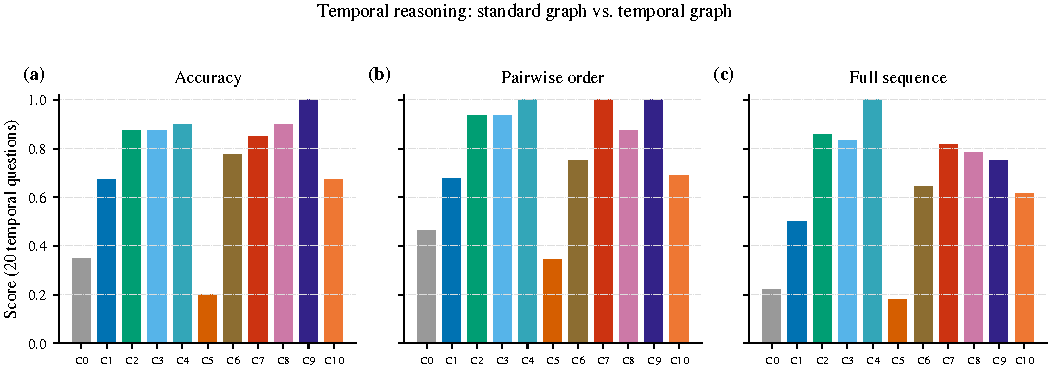
\includegraphics[width=\textwidth]{figures/fig4_temporal.pdf}
\caption{20 道时序题的正确率、pairwise order 与 full-sequence 正确率。C9 加入事件时间线与 \texttt{before} 边；C10 只按叙述顺序重排召回 chunk。}
\label{fig:temporal}
\end{figure}

\begin{table}[H]
\centering
\caption{时序题（20 题）的正确率、pairwise 顺序、全序与时长正确率。}
\label{tab:temporal}
\small
\begin{threeparttable}
\begin{tabular}{@{}l r c c c c@{}}
\toprule
Condition & $n$ & Accuracy & Pairwise order & Full sequence & Duration \\
\midrule
C0 & 20 & 0.35 & 0.46 & 0.22 & 0.00 \\
C1 & 20 & 0.68 & 0.68 & 0.50 & 0.67 \\
C2 & 20 & 0.88 & 0.94 & 0.86 & 1.00 \\
C3 & 20 & 0.88 & 0.94 & 0.83 & 1.00 \\
C4 & 20 & 0.90 & 1.00 & 1.00 & 1.00 \\
C5 & 20 & 0.20 & 0.35 & 0.18 & 0.00 \\
C6 & 20 & 0.78 & 0.75 & 0.64 & 1.00 \\
C7 & 20 & 0.85 & 1.00 & 0.82 & 1.00 \\
C8 & 20 & 0.90 & 0.88 & 0.79 & 1.00 \\
C9 & 20 & 1.00 & 1.00 & 0.75 & 1.00 \\
C10 & 20 & 0.68 & 0.69 & 0.62 & 0.67 \\
\bottomrule
\end{tabular}
\begin{tablenotes}\scriptsize
\item pairwise 与全序分数由评判模型的 \texttt{order\_results} 计算，标记为 \texttt{unclear} 的事件对不计入 pairwise 分母。Duration 为 Q18--Q20 三道时长题的正确率。
\end{tablenotes}
\end{threeparttable}
\end{table}


需要强调，C9 的时间线是按诗节人工整理的事件序列（55 个事件、54 条 \texttt{before} 边），与时序 gold 的判断来自同一首诗、同一标注者。C9 的 1.00 应理解为“有时序表示时的性能上限”，而非“自动时序抽取已经解决”。H3 的总体判定为部分支持，标准图并非在时序题上普遍更弱；显式时序结构能把时序题从 0.88 提高到 1.00，仅靠排序元数据（C10）则无效。

\subsection{H4 评测稳健性与部署成本}

人工盲审（44 条，条件标签隐藏）与第一评判模型的一致率为 0.727，二次加权 Cohen's $\kappa=0.797$\citep{cohen1960kappa}，严格二分类 $\kappa=0.535$，Spearman $\rho=0.845$。评判模型的平均 correctness 为 1.57，人工为 1.30，评判模型系统性偏宽松，在闭卷 C0（人工 0.0，评判模型 0.5）与空画像 C6（人工 1.25，评判模型 2.0）上最明显。绝对正确率因此应谨慎解读；条件间排序大体保留（$\rho=0.845$），且本文所有主指标都给出 bootstrap CI 与配对检验。第二评判模型（Llama-3.1-8B）在 220 条分层子集上与第一评判模型的总体一致率为 0.823，二次加权 $\kappa=0.531$，严格 $\kappa=0.438$，Spearman $\rho=0.570$。分条件看，C1/C4/C10 的 $\kappa$ 分别为 0.881/0.898/1.000，C5/C7 为 0.706/0.732；闭卷 C0 的 $\kappa$ 只有 0.047（Qwen 判 13 个 0、6 个 1、1 个 2；Llama 判 17 个 2、3 个 1），C2/C3/C6/C8/C9 在一个评判模型上出现常量评分（$\kappa$ 退化为 0，原始一致率仍为 0.85--0.95）。评判模型一致性在低质量答案上最脆弱，单评判模型的绝对分数不能视为稳定的 ground truth。

\begin{figure}[H]
\centering
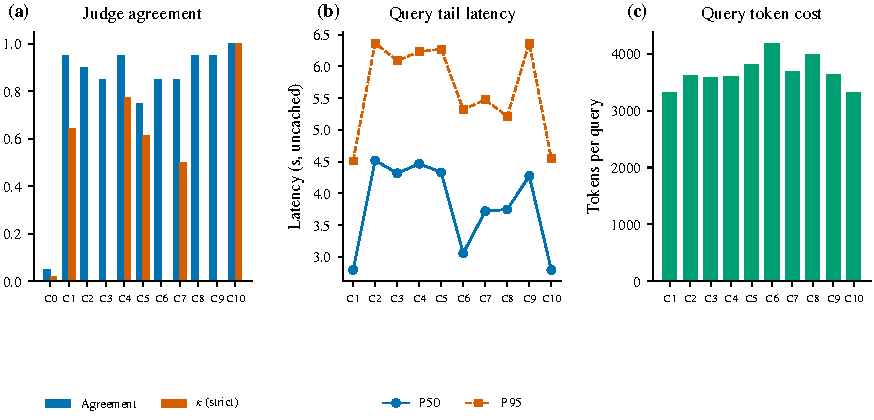
\includegraphics[width=\textwidth]{figures/fig5_cost_judge.pdf}
\caption{评测稳健性与部署成本。(a) 双评判模型一致率与严格 $\kappa$。(b) 查询尾延迟（P50/P95，未命中缓存）。(c) 每 query token。}
\label{fig:cost}
\end{figure}

\begin{table}[H]
\centering
\caption{双评判模型一致性（Qwen2.5-7B 与 Llama-3.1-8B）。}
\label{tab:judge}
\small
\begin{threeparttable}
\begin{tabular}{@{}l r c c c c@{}}
\toprule
Condition & $n$ & Agreement & $\kappa$ (quadratic) & $\kappa$ (strict) & Spearman $\rho$ \\
\midrule
C0 & 20 & 0.05 & 0.05 & 0.02 & 0.30 \\
C1 & 20 & 0.95 & 0.88 & 0.64 & 0.73 \\
C2 & 20 & 0.90 & 0.00 & 0.00 & -- \\
C3 & 20 & 0.85 & 0.00 & 0.00 & -- \\
C4 & 20 & 0.95 & 0.90 & 0.77 & 0.82 \\
C5 & 20 & 0.75 & 0.71 & 0.62 & 0.73 \\
C6 & 20 & 0.85 & 0.00 & 0.00 & -- \\
C7 & 20 & 0.85 & 0.73 & 0.50 & 0.63 \\
C8 & 20 & 0.95 & 0.00 & 0.00 & -- \\
C9 & 20 & 0.95 & 0.00 & 0.00 & -- \\
C10 & 20 & 1.00 & 1.00 & 1.00 & 1.00 \\
\bottomrule
\end{tabular}
\begin{tablenotes}\scriptsize
\item 一致率为 0/1/2 标签完全相同的比例，$\kappa$（二次加权）把 correctness 视为有序变量，$\kappa$（严格）把 correctness 2 视为阳性。若某个评判模型在该子集上为常量，$\kappa$ 退化为 0，Spearman 无法定义，表中以 --- 表示。
\end{tablenotes}
\end{threeparttable}
\end{table}


\begin{table}[H]
\centering
\caption{查询成本与延迟（未命中缓存；本地 RTX 5060，8GB）。}
\label{tab:cost}
\scriptsize
\setlength{\tabcolsep}{2.8pt}
\begin{threeparttable}
\begin{tabular}{@{}l r r r r r r r r@{}}
\toprule
Condition & $n$ & LLM calls & Prompt tok. & Completion tok. & Total tok. & P50 (s) & P95 (s) & Ctx tok. \\
\midrule
C0 & 100 & 1 & 100 & 99 & 199 & 2.05 & 2.91 & -- \\
C1 & 100 & 1 & 3248 & 63 & 3312 & 2.79 & 4.51 & 2862 \\
C2 & 100 & 2 & 3340 & 65 & 3614 & 4.52 & 6.37 & 2853 \\
C3 & 100 & 2 & 3299 & 68 & 3576 & 4.32 & 6.09 & 2830 \\
C4 & 100 & 2 & 3316 & 66 & 3590 & 4.47 & 6.23 & 2849 \\
C5 & 100 & 2 & 3557 & 50 & 3815 & 4.33 & 6.27 & 2900 \\
C6 & 100 & 2 & 3896 & 72 & 4176 & 3.06 & 5.32 & 2846 \\
C7 & 100 & 2 & 3404 & 74 & 3686 & 3.72 & 5.48 & 2849 \\
C8 & 99 & 2 & 3705 & 70 & 3983 & 3.75 & 5.21 & 2845 \\
C9 & 99 & 2 & 3366 & 63 & 3637 & 4.28 & 6.37 & 2854 \\
C10 & 100 & 1 & 3248 & 65 & 3313 & 2.79 & 4.55 & 2862 \\
\bottomrule
\end{tabular}
\begin{tablenotes}\scriptsize
\item token 为每 query 均值，延迟包含关键词抽取、检索与生成。C0 为闭卷（一次调用），C1/C10 一次，图条件两次（关键词与答案）。
\end{tablenotes}
\end{threeparttable}
\end{table}


全生命周期成本远高于原论文仅报告的“检索阶段 <100 token、一次调用”。索引阶段 28 次 LLM 调用、19,067 prompt token 与 13,410 completion token，合计 32,477 token，调用墙钟合计 195.8 秒；查询阶段 C2 平均约 3,614 token、P50 4.52 秒、P95 6.37 秒，C1 为 3,312 token、2.79/4.51 秒。图条件每 query 需要两次 LLM 调用（关键词与答案），NaiveRAG 一次。增量更新（前 14 chunk 已索引，追加后 14 chunk）只需 15,949 token，相对全量 32,477 token 节省 50.9\%。存储为图 JSON 166 KB、时序图 222 KB、C2 画像 195 KB、C8 画像 189 KB、embedding 约 10.4 MB。H4 的判定为支持；单一 LLM 评判模型偏宽松、缺少 CI 的评测，以及仅计检索阶段 token 的成本口径，都会高估方法质量并低估部署成本。

\subsection{判定汇总}

\begin{table}[H]
\centering
\caption{四个批评点的判定汇总。}
\label{tab:verdict}
\small
\begin{tabular}{@{}p{0.08\textwidth}p{0.58\textwidth}p{0.24\textwidth}@{}}
\toprule
假设 & 关键证据 & 判定\\
\midrule
H1 & C2$-$C1 $+0.025$ ($p=0.515$)；C2$-$C6 $+0.005$；C2$-$C7 $+0.015$；C2$-$C5 $+0.400$ ($p<0.001$) & 支持（图与画像无显著增益；原文是关键）\\
H2 & LLM 画像支持率 0.952/0.871 对抽取式 0.883/0.877；C2$-$C8 三项均不显著；ROUGE-L 0.020/0.026 对 0.030/0.055 & 部分支持（字面漂移成立，事实偏差未证实）\\
H3 & C2 时序 0.88 不低于非时序；C2$-$C1 时序 $+0.200$ ($p=0.005$)；C9$-$C2 $+0.125$ ($p=0.077$)；C9$-$C10 $+0.325$ ($p<0.001$) & 部分支持（时序结构有效，但标准图并非普遍失效）\\
H4 & 人工 $\kappa_3=0.797$、严格 $\kappa=0.535$；评判模型均值 1.57 对人工 1.30；C2 每 query 3.6k token、P50 4.5 s & 支持（单评判模型偏宽松；全生命周期成本更高）\\
\bottomrule
\end{tabular}
\end{table}